\documentclass{sigkdd}
\usepackage{blindtext}

\usepackage{color}
\usepackage{tikz}
\usetikzlibrary{arrows}
\usepackage{chngcntr}



\title{Message Passing and Expectation Propagation}
\subtitle{Efficient Inference in large scale machine learning}
\numberofauthors{1}
\author{
\alignauthor Christoph Dehner \\
\affaddr{Department of Informatics}\\
\affaddr{Technische Universit\"at M\"unchen}\\
\email{dehner@in.tum.de}
}
\counterwithout{equation}{section}

\begin{document}
\maketitle

% Abstract
\begin{abstract}
This paper explains two efficient Bayesian inference methods basing on a factorized version of a joint probability distribution. The two message passing algorithms "Max-sum" and Sum-product" enable exact inference in tree-shaped graphical models. The underlying concept of message passing can also be generalized to arbitrary graphs.

By expectation propagation a second approximate inference technique is covered. Similarly to variational inference it aims at minimizing the KL divergence of an approximating distribution. This is done in an iterative way leading to a useful approximate inference method for many situations.
\end{abstract}

\section{Introduction}
Probabilistic graphical models like Markov Random Fields or Bayesian Networks provide clear and illustrative ways to describe probabilistic processes. In such models, nodes represent random variables and edges their conditional dependencies. The joint distribution of all involved variables can be expressed as a product of factors, which are observed or given specific values during modeling. As an example, a Bayesian network with three variables is given in figure \ref{fig:BN}. It defines the values of $x_1$ and $x_3$ to be conditionally independent given $x_2$.
\begin{figure}[h]
	\centering
	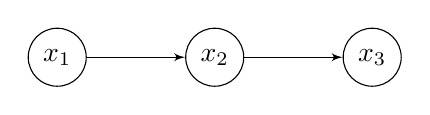
\begin{tikzpicture}
	
	\tikzset{vertex/.style = {shape=circle,draw,minimum size=1.5em}}
	\tikzset{edge/.style = {->,> = latex'}}
	
	\node[vertex] (x1) at  (0,0) {$x_1$};
	\node[vertex] (x2) at  (2,0) {$x_2$};
	\node[vertex] (x3) at  (4,0) {$x_3$};
	
	\draw[edge] (x1) to (x2);
	\draw[edge] (x2) to (x3);
	\end{tikzpicture}
	\caption{Bayesian network with three variables. $x_1$ and $x_3$ are conditionally independent given $x_2$.}\label{fig:BN}
\end{figure}

Typical tasks in such a scenario are to do Bayesian inference to extract marginal distributions of specific variables or find maximum aposteriori estimates. However, with an increasing number of variables these task can become computationally very expensive. 

The naive approach for marginalization is to sum out all but one variable from the joint distribution $p(X)$. This is formally shown in equation \ref{eq:marginalisation_naive}, where $X \setminus x_i$ describes the set of all random variables except $x_i$.
This strategy requires exponentially many evaluations of the joint distribution in the number of variables and is thus not applicable to bigger networks.
\begin{equation}\label{eq:marginalisation_naive}
p(x_i)= \sum_{X \setminus x_i} p(X)
\end{equation}
Therefore, this paper explains more efficient algorithms to do large scale Bayesian inference in graphical models. Chapter \ref{chapter:exact_inference} deals with message passing and presents two belief propagation algorithms to calculate exact marginals and maximum aposteriori estimates for tree-shaped graphical models. Furthermore, generalized message passing approaches for arbitrary graphs are presented at the end of the chapter. Subsequently, in chapter \ref{chapter:approximate_inference} expectation propagation as a method of approximate inference is explained.

Before the different inference approaches are explained in detail, the next section introduces factor graphs, the structure these algorithms operate on.

\section{Factor graphs}
Factor graphs make the factorization of a joint probability distribution explicit. The can be generated from Bayesian networks as well as from Markov random fields and thus allow to define inference algorithms independent of how the underlying probabilistic graphical model was introduced.

Additional to the variable nodes, a factor graph also consists of factor nodes representing the factors of the decomposed joint probability distribution as in equation  \ref{eq:product_of_factors}. Edges connect the factor nodes to all variables they depend on. By this way they form a bipartite graph with variable nodes (usually visualizes by circles) on the one side and and factors (depicted as rectangles) on the other side.

Depending on the exact factorization, a distribution defined by a Bayesian network or Markov random field can be represented by different factor graphs. Figure \ref{fig:FG} depicts a factor graph of the Bayesian network from figure \ref{fig:BN}, in which all conditional distributions are represented by separate factors.

\begin{figure}[h]
	\centering
	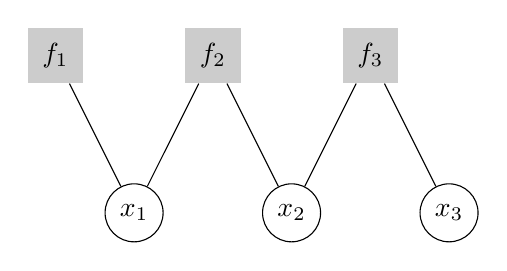
\begin{tikzpicture}
	
	\tikzset{vertex/.style = {shape=circle,draw,minimum size=1.5em}}
	\tikzset{edge/.style = {-,> = latex'}}
	
	\node[vertex] (x1) at  (0,0) {$x_1$};
	\node[vertex] (x2) at  (2,0) {$x_2$};
	\node[vertex] (x3) at  (4,0) {$x_3$};
	
	\tikzset{vertex/.style = {shape = rectangle,fill = gray!40,minimum size=2em}}
	\node[vertex] (f1) at  (-1,2) {$f_1$};
	\node[vertex] (f2) at  (1,2) {$f_2$};
	\node[vertex] (f3) at  (3,2) {$f_3$};
	
	\draw[edge] (x1) to (f1);
	\draw[edge] (x1) to (f2);
	\draw[edge] (x2) to (f2);
	\draw[edge] (x2) to (f3);
	\draw[edge] (x3) to (f3);
	\end{tikzpicture}
	\caption{Factor graph of the Bayesian network from figure \ref{fig:BN}. The factors $f_1$, $f_2$ and $f_3$ correspond to the probability distributions $p(x_1)$, $p(x_2|x_1)$ and $p(x_3|x_2$.)}\label{fig:FG}
\end{figure}

The inference algorithms on factor graphs of the following section are valid for trees. Such factor graphs with exactly one path between any pair of nodes can be generated from undirected trees in the case of a Markov random field model as well as from from directed trees and polytrees, if the factor graph is derived from a Bayesian network. More detailed descriptions of how to derive factor graph from probabilistic graph models can be found in \cite{bishop2006prml}.\footnote{Chapter 8.3.2 for the moralization step of undirected models and chapter 8.4.3 for the concrete buildup of a factor graph from a graphical model.}

\section{Message passing}\label{chapter:exact_inference}
The intuition of the algorithms presented in this section is to exploit independence properties of the random variables. Graphical models define the joint probability to be expressed as a product of factors, considering the conditional independences expressed by the graph. For Bayesian networks those factors correspond to conditional distributions, in Markov Random Fields to clique potentials. Assuming appropriately normalized factors, the joint distribution can be written as a product according to equation \ref{eq:product_of_factors}. The index $s$ iterates here over all factors of the graph; $X_s$ defines the subset of variables, the factor $s$ depends on.
\begin{equation}\label{eq:product_of_factors}
p(X)= \prod_{s} f_s(X_s)
\end{equation}
Expressing the joint distribution as the product defined by the graph allows to exchange summations and multiplications during marginalization. By this way, marginalization can often be done a lot more efficient. Equation \ref{eq:marginalization_smart} demonstrates this transformation with the Bayesian network from figure \ref{fig:BN}, whose joint distribution $p(X)$ is defined as $p(X) =  p(x_1) p(x_2|x_1) p(x_3|x_1)$.
\begin{equation}\label{eq:marginalization_smart}
\begin{split}
p(x_2) &= \sum_{x_1} \sum_{x_3} p(x_1) p(x_2|x_1) p(x_3|x_2) \\ &= \sum_{x_1} \Big[  p(x_1) p(x_2|x_1) \sum_{x_3} \Big[ p(x_3|x_2)\Big] \Big] \\ &= \underbrace{\Big[ \sum_{x_1}  p(x_1) p(x_2|x_1)\Big]}_{\mu_{x_1 \rightarrow x_2}}\cdot \underbrace{\Big[ \sum_{x_3}  p(x_3|x_2)\Big]}_{\mu_{x_3 \rightarrow x_2}}
\end{split}
\end{equation}
Here, the sum of products from the naive approach for marginalization is transformed to a product of sums, reducing the exponential computational complexity in the number of random variables to linear effort.

The brackets in the last line of equation \ref{eq:marginalization_smart} reveal a powerful interpretation of the marginalizing. The marginal distribution $p(x_2)$ consists of two messages $\mu_{x_1 \rightarrow x_2}$ and $\mu_{x_3 \rightarrow x_2}$ from its neighboring cells $x_1$ and $x_3$. For a longer chain of random variables these messages would again be comprised by messages from their neighboring cell. Applied to a chain of arbitrary length, this method gives a recursive pattern in which messages for the marginalization are sent to the marginalized variable node from both ends of the chain.  

This message passing idea is the foundation for the two inference algorithms presented in this chapter subsequently.


\subsection{Sum-product algorithm}
The sum-product algorithm presented in this section generalizes the idea of exchanging summation and multiplication during marginalization. It consists of local messages passed between factor and variable nodes in a factor graph.

As a starting point let us consider the calculation of the marginal distribution $p(x_i)$ in the factor graph of figure \ref{fig:message1}. Furthermore we define $F_s(s, X_s)$ for all neighbors $s$ of $x_i$ as the product of all factors in the respective sub-tree of the neighbor. This is visualized by green circles in figure \ref{fig:message1}.
\begin{figure}[h]
	\centering
	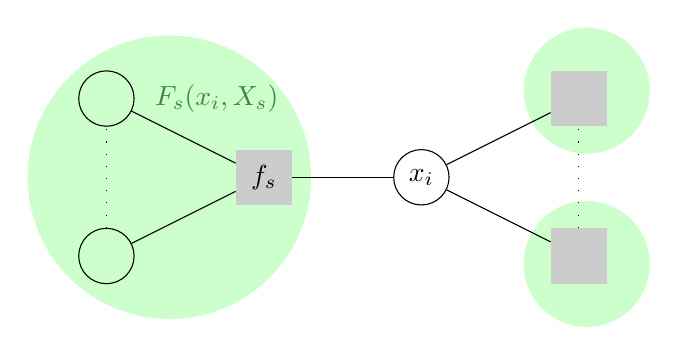
\begin{tikzpicture}
	
	\definecolor{darkgreen}{RGB}{59,136,59}
	
	\tikzstyle{edge} = [draw,-]
    \fill[green!20]   (0:-1.2) circle (1.8);
    \node[darkgreen] (text) at (-0.6,1) {$F_s(x_i,X_s)$};
    
    \fill[green!20]   (4.1,-1.1) circle (0.8);
    \fill[green!20]   (4.1,1.1) circle (0.8);

	\tikzset{vertex/.style = {shape=circle,draw,minimum size=2em}}
	\node[vertex] (xi) at  (2,0) {$x_i$};
	\node[vertex] (xl1) at  (-2,-1) {};
	\node[vertex] (xl2) at  (-2,1) {};
	
	\tikzset{vertex/.style = {shape = rectangle,fill = gray!40,minimum size=2em}}
	\node[vertex] (fs) at  (0,0) {$f_s$};
	\node[vertex] (xr1) at  (4,-1) {};
	\node[vertex] (xr2) at  (4,1) {};
	
	\draw[edge] (fs) to (xi);
	\draw[edge] (xi) to (xr1);
	\draw[edge] (xi) to (xr2);
	\draw[edge] (fs) to (xl1);
	\draw[edge] (fs) to (xl2);
	\draw[edge, loosely dotted] (xr1) to (xr2);
	\draw[edge, loosely dotted] (xl1) to (xl2);
	\end{tikzpicture}
	\caption{Exemplary factor graph to visualize the deduction of an expression for the marginal distribution of $x_i$ in equation \ref{eq:message1}. The green circles define for all neighbors of $x_i$ the product of all factors in the respective sub-tree and support the expression of the joint distribution in equation \ref{eq:product_of_neighbours}.}\label{fig:message1}
\end{figure}

Analogously to the general factorization defined by the graphical model from equation \ref{eq:product_of_factors} the joint probability $p(X)$ can then be expressed as a product of those neighbor-factors of $x_i$:
\begin{equation}\label{eq:product_of_neighbours}
p(X)= \prod_{s \in ne(x_i)} F_s(x_i, X_s)
\end{equation}
Inserting this representation of the joint distribution in the naive marginalization formula from equation \ref{eq:marginalisation_naive} allows to exchange sum and product. By this way the marginal distribution of $x_i$ is expressed as the product of messages $\mu_{f_s \rightarrow x_i}$ from all its neighbors in the factor graph:
\begin{equation}\label{eq:message1}
\begin{split}
p(x_i) &= \sum_{X \setminus x_i} \Big[ \prod_{s \in ne(x_i)} F_s(x_i, X_s) \Big] \\ &= \prod_{s \in ne(x_i)} \Big[ \sum_{X_s} F_s(x_i, X_s)\Big] =: \prod_{s \in ne(x_i)} \mu_{f_s \rightarrow x_i}(x_i)
\end{split}
\end{equation}

The factors $F_s(x,X_s)$ represent subtrees in the factor graph and can thus be factorized again: 
\begin{equation}\label{eq:product2}
F_s(x_i,X_s) = f_s(x_i, X_s) G_1(x_1, X_{s_1})\dots G_1(x_M, X_{s_M}).
\end{equation}
The factors $G_1(x_1, X_{s_1})\dots G_1(x_M, X_{s_M})$ represent here the subgraphs of all neighbors of $f_s$ except from $x_i$ and are illustrated by red circles in figure \ref{fig:message2}.

\begin{figure}[h]
	\centering
	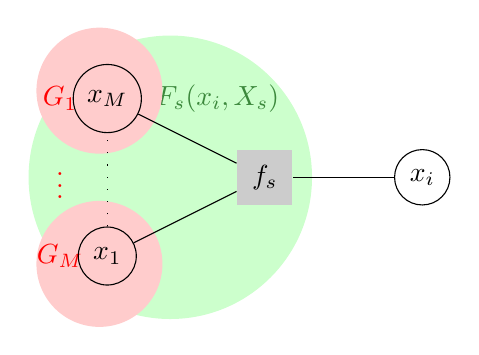
\begin{tikzpicture}
	
	\definecolor{darkgreen}{RGB}{59,136,59}
	
	\tikzstyle{edge} = [draw,-]
    \fill[green!20]   (0:-1.2) circle (1.8);
    \node[darkgreen] (text) at (-0.6,1) {$F_s(x_i,X_s)$};
    
    \fill[red!20]   (-2.1,-1.1) circle (0.8);
    \fill[red!20]   (-2.1,1.1) circle (0.8);
    \node[red] (text) at (-2.6,1) {$G_1$};
    \node[red] (text) at (-2.6,0) {$\vdots$};
    \node[red] (text) at (-2.6,-1) {$G_M$};


	\tikzset{vertex/.style = {shape=circle,draw,minimum size=2em}}
	\node[vertex] (xi) at  (2,0) {$x_i$};
	\node[vertex] (xl1) at  (-2,-1) {$x_1$};
	\node[vertex] (xl2) at  (-2,1) {$x_M$};
	
	\tikzset{vertex/.style = {shape = rectangle,fill = gray!40,minimum size=2em}}
	\node[vertex] (fs) at  (0,0) {$f_s$};
	
	\draw[edge] (fs) to (xi);
	\draw[edge] (fs) to (xl1);
	\draw[edge] (fs) to (xl2);
	\draw[edge, loosely dotted] (xl1) to (xl2);
	\end{tikzpicture}
	\caption{Exemplary factor graph to visualize the deduction of an expression for messages from factors to nodes equation \ref{eq:message2}. The red circles represent the factorization expressed in equation  \ref{eq:product2}.}\label{fig:message2}
\end{figure}

With that, the messages defined in equation \ref{eq:message1} can be further evaluated to
\begin{equation}\label{eq:message2}
\begin{split}
\mu_{f_s \rightarrow x_i}(x_i) &= \sum_{X_s \setminus x_i} f_s(x_i, X_s) \prod_{m \in ne(f_s) \setminus x_i} \Big[ \sum_{{X_s}_m} G_m(x_m, {X_s}_m)  \Big] \\ &= \sum_{\mathbf{x_s} \setminus x_i} f_s(x_i, X_s) \prod_{m \in ne(f_s) \setminus x_i} \mu_{x_m \rightarrow f_s}(x_m).
\end{split}
\end{equation}
We have now defined  messages from factor to variable nodes. $\mu_{x_m \rightarrow f_s}(x_m) :=\sum_{{X_s}_m} G_m(x_m, {X_s}_m)$. Going one step further yields an expression for messages from variables to factors as well. Analogously to before, $G_m(x_m, {X_s}_m)$ can be factorized again to 
\begin{equation}\label{eq:product3}
G_m(x_m,{X_s}_m) = \prod_{l \in ne(x_m) \setminus f_s} F_l(x_m, {{X_s}_m}_l),
\end{equation}
as visualized in figure \ref{fig:message3}. The factors $F_l$ are visualized by blue circles.

\begin{figure}[h]
	\centering
	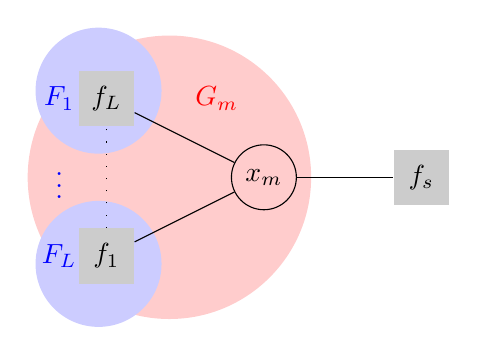
\begin{tikzpicture}
	
	\definecolor{darkgreen}{RGB}{59,136,59}
	
	\tikzstyle{edge} = [draw,-]
    \fill[red!20]   (0:-1.2) circle (1.8);
    \node[red] (text) at (-0.6,1) {$G_m$};
    
    \fill[blue!20]   (-2.1,-1.1) circle (0.8);
    \fill[blue!20]   (-2.1,1.1) circle (0.8);
    \node[blue] (text) at (-2.6,1) {$F_1$};
    \node[blue] (text) at (-2.6,0) {$\vdots$};
    \node[blue] (text) at (-2.6,-1) {$F_L$};

	\tikzset{vertex/.style = {shape = rectangle,fill = gray!40,minimum size=2em}}
	\node[vertex] (xi) at  (2,0) {$f_s$};
	\node[vertex] (xl1) at  (-2,-1) {$f_1$};
	\node[vertex] (xl2) at  (-2,1) {$f_L$};
	
	\tikzset{vertex/.style = {shape=circle,draw,minimum size=2em}}
	\node[vertex] (fs) at  (0,0) {$x_m$};
	
	\draw[edge] (fs) to (xi);
	\draw[edge] (fs) to (xl1);
	\draw[edge] (fs) to (xl2);
	\draw[edge, loosely dotted] (xl1) to (xl2);
	\end{tikzpicture}
	\caption{Exemplary factor graph to visualize the deduction of an expression for messages from nodes to factors equation \ref{eq:message3}. The blue circles represent the factorization expressed in equation  \ref{eq:product3}.}\label{fig:message3}
\end{figure}

Inserting this factorization into the definition of $\mu_{x_m \rightarrow f_s}(x_m)$ and exchanging summation and multiplication reveals an explicit formula for this messages:
\begin{equation}\label{eq:message3}
    \begin{split}
        \mu_{x_m \rightarrow f_s}(x_m) &=\sum_{{X_s}_m} \Big[ \prod_{l \in ne(x_m) \setminus f_s} F_l(x_m, {{X_s}_m}_l) \Big] \\ &= \prod_{l \in ne(x_m) \setminus f_s} \Big[\sum_{{{X_s}_m}_l} F_l(x_m, {{X_s}_m}_l) \Big] \\ &= \prod_{l \in ne(x_m) \setminus f_s} \mu_{f_l \rightarrow x_m}(x_m)
    \end{split}
\end{equation}

We have now induced how a marginal distribution $p(x_i)$ can be expressed by local messages passed between factors and variables through the factor graph. For leave nodes those messages can be stated explicitly.
In case a variable node is leave of the factor graph, equation \ref{eq:message3} shows that the message, the node sends to its only neighbor, is given by
\begin{equation}\label{eq:marg_init_1}
\mu_{x \rightarrow f}(x) = 1.
\end{equation}
Similarly, from equation \ref{eq:message2} then concludes the initial value
\begin{equation}\label{eq:marg_init_2}
\mu_{f \rightarrow x}(x) = f(x)
\end{equation}
for a message from a leave factor node to its neighboring variable node.

Having explicit start values for messages from the leaves, messages can propagated through the factor graphs to an arbitrarily chosen root node. This root node has then received messages from all its neighbors and can thus calculate its marginal distribution according to \ref{eq:message1}. Analogously, passing all messages back from the root to all leave nodes enables to calculate the marginals of all variables in the factor graph. For this calculation two times the number of edges in the factor graph many messages have to be computed, which is linear in the number of variables of the model.\\

\subsection{Max-sum algorithm}
Next to computing marginal distributions, a frequent task is to find maximum a posteriori estimates. The aim is to finding values for all random variables, which maximize the joint probability distribution. This can be formulated mathematically as
\begin{equation}\label{eq:map_problem}
X^* = \underset{X}{\arg\max}~ p(X) = \underset{X}{\arg\max}~ \ln (p(X)).
\end{equation}
The value for the maximal joint probability is given by
\begin{equation}\label{eq:map_problem2}
p(X^*) = \underset{X}{\max}~ \ln (p(X)).
\end{equation}


The actual algorithm works similarly to the sum-product algorithm from the previous chapter, but with the exception that maximizations instead of sums over the random variables are performed. Analogously to before, the idea behind is to insert the factorized expression of the joint distribution from equation \ref{eq:product_of_neighbours} into the problem formulation from equation \ref{eq:map_problem2} and exchange maximization and multiplication.

The second step of equation \ref{eq:map_problem} contains a transformation, which allows a simplification. Since the logarithm is a strictly monotonic increasing function, it does not change the optimum $X^*$ but transforms the products in the messages to sums. Thus, the algorithm derived in this section is not called "max-product", which the analogy to the "sum-product" algorithm from the previous section would suggest, but "max-sum" algorithm.

Applying all discussed modification to the formulas deduced in the last chapter leads to the following messages:
\begin{equation}\label{eq:map_m1}
\begin{split}
\mu_{f_s \rightarrow x_i}(x_i) = \max_{X_s \setminus x_i} \Big[f_s(x_i, X_s) \sum_{m \in ne(f_s) \setminus x_i} \mu_{x_m \rightarrow f_s}(x_m) \Big]
\end{split}
\end{equation}

\begin{equation}\label{eq:map_m2}
\begin{split}
\mu_{x_m \rightarrow f_s}(x_m) = \sum_{l \in ne(x_m) \setminus f_s} \mu_{f_l \rightarrow x_m}(x_m)
\end{split}
\end{equation}

Also the message initializations for leave nodes from equation \ref{eq:marg_init_1} and \ref{eq:marg_init_2} must be adjusted with the logarithm, resulting in
\begin{equation}\label{eq:marg_init2_1}
\mu_{x \rightarrow f}(x) = 0,
\end{equation}
\begin{equation}\label{eq:marg_init2_2}
\mu_{f \rightarrow x}(x) = \ln(f(x)).
\end{equation}
By propagating messages from all leave nodes to an arbitrarily chosen root node, the maximal value of the joint probability distribution can be calculated in that root node. The message passing is again done in a fashion, that a node can forward its message to its parent node as soon it has received messages from all children.

The missing step is to find the variable configuration for the maximal joint probability. The central maximization is performed in equation \ref{eq:map_m1} over the variables of each factor before its message is passed further to the root. By saving the maximal configuration of each factor at this step, the values of the variables which give rise to the maximal joint probability can be obtained. In contrast to the sum-product algorithm, the max-sum algorithm does not require to propagate messages back from the root to all leaves.

\subsection{Discussion}
The two algorithms require a fixed number of passes through the graph. Thus their computational complexity depends on the number of edges, which increases linearly with the number of involved random variables. Next to this factor, the computational cost of the two algorithms also consists a polynomial factor in the number of values, the discrete random variables can take.

The big disadvantage of the sum-product and max-sum algorithms is that they only work on trees-shaped graphical models. To overcome this, the next section presents approaches to overcome this and do inference via message passing in general graphs.

\subsection{Inference via message passing in general graphs}
The discussed inference methods only produce valid results for trees. However, since the algorithms only consist of local messages passed through the graph, they can also be applied to graphs which contain circles. This is called "loopy belief propagation". For that, all messages need to be initialized by the unit function and a message passing schedule must be defined to state the order in which the messages are passed through the graph.

With circles in the graph, loopy belief propagation is not guaranteed to converge. In some situations it produces only poor results, while in other situations the final outcome turned out to be quite accurate. Certain error-correcting codes for example are equivalent to loopy belief propagation.

There are also algorithms, which generalize the message passing idea to work for arbitrary graphs. The junction tree algorithm resolves circles in a general graph by a triangulation step and extraction of a maximal spanning tree. Depending on the underlying graph the algorithm requires exponential effort, but is efficient from the perspective that there are generally no cheaper approaches for exact inference in arbitrary graphs.

Linearized belief propagation is another approach to overcome loops in the graph. By restricting the values to be close to certain default values, the problem can be formulated in a matrix framework, for which there is a closed-form solution. More information can be found in \cite{Gatterbauer:2015:LSB:2735479.2735490}. 

\section{Expectation propagation}\label{chapter:approximate_inference}
This chapter presents by expectation propagation (EP) a method for approximate inference. In the following section the methodology behind and the concrete algorithm are explained at first. Secondly, some interesting properties when applying expectation propagation to graphical models are highlighted. At last, a general discussion and comparison to variational inference is given.

\subsection{Methodology}
Similarly to variational inference (VI), in EP the true distribution $p(\mathbf{z})$ of a model is approximated by a simpler distribution $q(\mathbf{z})$. The approximation is computed and measured by minimizing the Kullback-Leibler divergence of the two functions. However, while in VI $KL(q||p)$ is considered, EP swaps the distributions and aims at minimizing $KL(p||q)$.

For $q(\mathbf{z})$ a member of the exponential family with the form
\begin{equation}\label{eq:ep1}
q(\mathbf{z}) = h(\mathbf{z})g(\mathbf{\eta}) \exp(\mathbf{\eta}^T(u(\mathbf{z})))
\end{equation}
must be chosen. With that the KL divergence becomes
\begin{equation}\label{eq:ep2}
KL(p||q)= - \ln g(\eta) - \eta^T \mathbf{E}_{p(\mathbf{z})} [u(\mathbf{z})] + const.
\end{equation}
The distribution $q(\mathbf{z})$, which minimizes this KL divergence from equation \ref{eq:ep2}, can be constructed by moment matching. If $q(\mathbf{z})$ is a Gaussian for example, its mean corresponds to the mean of $p(\mathbf{z})$ and its covariance is equal to the covariance of $p(\mathbf{z})$.

\subsection{Expectation propagation algorithm}
For the concrete EP algorithm we consider a model of hidden variables and parameters $\theta$ and observed data $\mathbf{D}$. Similarly to the previous chapter we assume that the joint distribution can be written as a product of factors $f_i$. However, one factor is not restricted to depend on only a subset of variables here, but has all latent variables and parameters (together represented by $\theta$) as its arguments.
\begin{equation}\label{eq:ep3}
p(\theta, \mathbf{D}) = \prod_i f_i(\theta).
\end{equation}
The goal is then to approximate the posterior distribution $p(\theta|\mathbf{D})$, which can be expressed by the joint distribution and the evidence $p(\mathbf{D})$:
\begin{equation}\label{eq:ep4}
p(\theta|\mathbf{D}) = \frac{1}{p(\mathbf{D})} \prod_i f_i(\theta , \mathbf{D}),
\end{equation}
with 
\begin{equation}\label{eq:ep5}
p(\mathbf{D}) = \int \prod_i f_i(\theta) d\theta.
\end{equation}  

Adapting to the structure of the true posterior distribution, $q(\theta)$ is chosen as a product of factors $\tilde{f}_i$ from a exponential family, which each correspond to one of the true factors $f_i$. By this way, $q(\theta)$ is also from this exponential family. $\frac{1}{Z}$ represents the normalizing factor for the distribution:
\begin{equation}\label{eq:ep6}
q(\theta) = \frac{1}{Z}\prod_i \tilde{f}_i(\theta)
\end{equation}

The factors $\tilde{f}_i$ are refined iteratively. Starting with a rough initialization of all approximating factors $\tilde{f}_i$, in each iteration on factor is refined closer to its true factor $f_i$, while the rest of the factors are fixed. Assuming we want to refine factor $j$, we first define the product of the fixed factors $q^{\backslash j}(\theta)$ for that:
\begin{equation}\label{eq:ep7}
q^{\backslash j}(\theta) = \prod_{i\ne j} \tilde{f}_i(\theta)
\end{equation}
Then we evaluate a new approximation of the posterior $q^{new}(\theta)$ by matching the moments of $f_j \cdot q^{\backslash j}(\theta)$:
\begin{equation}\label{eq:ep7.1}
q^{new}(\theta) \propto f_j ~ q^{\backslash j}(\theta)
\end{equation}
Finally, we can extract and store a new approximation of $\tilde{f}_j$ from that. $\frac{1}{Z_j}$ again represents a necessary normalizing factor here:
\begin{equation}\label{eq:ep8}
\tilde{f}_j = \frac{1}{Z_j} \frac{q^{new}(\theta)}{q^{\backslash j}(\theta)}
\end{equation}

\subsection{Expectation propagation in graphical models}
Whereas general expectation propagation allows the factors of the joint distribution to depend on all parameters and latent variables of the model (see equation \ref{eq:ep4}), in graphical models the factors of the joint distribution depend on a subset of variables $\theta_i$:
\begin{equation}\label{eq:ep9}
p(\theta|\mathbf{D}) = \frac{1}{p(\mathbf{D})} \prod_i f_i(\theta_i),
\end{equation}
An interesting property gets visible if we use a fully factorized approximation function: Then, the EP algorithm becomes equal the sum-product algorithm. In other words, the sum-product algorithm turns out to be a special case of expectation propagation, if using fully independent variables in the approximation function.

With respect to the approximation function of the EP algorithm an interpretation can be formulated: Since the sum-product algorithm is an exact inference algorithm, a more flexible approximation function compared to the underlying model (as for example one with a few dependency connections in the graph left out) can increase the accuracy.

Another approach to incorporate some extent of generalization to expectation propagation is to refine a set of factors together within one iteration of the algorithm. However, for both methods there are still open research question how to find the best amount of independence for the approximation function of EP as well as the optimal grouping of factors for simultaneous refinement.

\subsection{Discussion}
A key disadvantage of expectation propagation is that is not guaranteed to converge. For the exponential family the resulting KL-divergence function is proven to have a stationary point, but the iteration of EP might not reach it.

Variational inference in contrast provides a lower bound in each optimization step and thus guarantees to converge. However, EP can nevertheless be a powerful inference method. Because variational inference operates with a lower bound it often underestimates the variance of the true distribution. Therefore, if expectation propagation converges, it often outperforms other variational methods.

On the other hand, if the algorithm does not converge, it might be for a good reason an the chosen exponential family approximates the true posterior only poorly.

Another aspect leading to conceptually different behavior between expectation propagation and variational inference comes from the approach how the KL divergence is minimized. Expectation propagation minimizes $KL(p||q)$, while variational inference aims at reducing $KL(q||p)$. For multimodal distribution this leads to significantly worse results for expectation propagation. Since the EP algorithm tries to incorporate all modes of the underlying probability distribution it can approximate function with more than one mode only badly. This is visualized in figure \ref{fig:multimodal}, which is taken from \cite{bishop2006prml}.

\begin{figure}[h]
	\begin{center}
		\includegraphics[scale=0.12]{multimodal_approximation.png}
		\caption{Approximation of a multimodal distribution by a) minimizing $KL(p||q)$, b) minimizing $KL(q||p)$ and c) same approach as b) but with a different result.}\label{fig:multimodal}
	\end{center}
\end{figure}
\section{Summary and outlook}
In summary, message passing as well as expectation propagation are useful inference methods. If the underlying graphical model is a tree, the max-sum and sum-product algorithm compute exact results in an efficient way.

For general models, there exist different approaches for approximate inference. Methods like loopy belief propagation or linearized belief propagation generalize the concept of message passing to arbitrary graphs. Expectation propagation follows an approach similar to variational inference and tries to find an approximation of the true distribution by minimizing the KL divergence.
However, none of these methods is in general superior. Depending on the concrete problem setting, either of the presented method can produce more accurate results.

There is also ongoing research about the discussed approaches, especially for message passing. \cite{Gatterbauer:2015:LSB:2735479.2735490} does not only present a linearized belief propagation but also shows an incremental version. Furthermore it describes a single-pass variation, in which only one message for each node is calculated.

Finally, as second outlook \cite{wayoflife} is presented. It considers Bayesian inference methods like expectation propagation on partitioned data. By this way, such inference methods could be applied to big data.


% Bibliography
\bibliographystyle{abbrv}
% Add references using the command below
\bibliography{references}
\nocite{*}
%\cite{Seeger05expectationpropagation}

\end{document}